\documentclass[conference]{IEEEtran}
\IEEEoverridecommandlockouts
% The preceding line is only needed to identify funding in the first footnote. If that is unneeded, please comment it out.
\usepackage{cite}
\usepackage{amsmath,amssymb,amsfonts}
\usepackage{algorithm}
\usepackage{algorithmic}
\usepackage{graphicx}
\usepackage{textcomp}
\usepackage{xcolor}
\usepackage{multirow}
\usepackage{multicol}
\usepackage{subfigure}
\usepackage{ntheorem}
\usepackage{enumerate}
\usepackage[bottom]{footmisc}
\usepackage{soul}

\usepackage[T1]{fontenc}
\usepackage{mathptmx}
\soulregister\cite7
\soulregister\ref7
\pagestyle{plain}

\def\BibTeX{{\rm B\kern-.05em{\sc i\kern-.025em b}\kern-.08em
    T\kern-.1667em\lower.7ex\hbox{E}\kern-.125emX}}
\begin{document}

\title{\LARGE{Approximate Code: A Cost-Effective Erasure Code for MultimediavApplications in Cloud Storage Systems}\\
}
\author{\IEEEauthorblockN{Huayi Jin$^1$}
}

\maketitle

\begin{abstract}
Erasure codes are commonly used to ensure data availability in cloud storage systems, where video data produced by autopilot, multimedia industry and security monitoring occupies large amounts of space.
Typical erasure codes, such as Reed-Solomon (RS) \cite{macwilliams1977theory} codes or XOR-based codes use several parity disks to equally back up all data.
However, this is expensive, not only because simultaneous damage of multiple disks is relatively rare, but also due to the ignorance of redundant information inside the data, which results in multiple complete parity disks being excessive.


Therefore, we propose Approximate Codes for video data, which significantly reduce storage overhead and increase availability for more important data segments.
Approximate Codes provide complete recovery when fewer disks fail, and ensure approximate recovery (recover most data) in the event of multiple disk failures.
To demonstrate the effectiveness of Approximate Codes, we conduct several experiments in Hadoop and Alibaba Cloud systems.
The results show that compared with the typical high-reliability erasure code schemes, Approximate Codes reduce the storage overhead by 7.64\% at the expense of reasonable probability of video quality loss.

\end{abstract}

\begin{IEEEkeywords}
    Erasure Codes, Approximate Storage, Multimedia, Cloud Storage
\end{IEEEkeywords}

\section{Introduction}
Currently, many cloud storage systems use erasure codes to tolerate disk failures and ensure data availability, such as Windows [], Amazon AWS [] or Alibaba Cloud. It is known that erasure codes provide much lower storage overhead and write bandwidth than replication with the same fault tolerance.

Typical erasure codes schemes can be divided into two categories such as RS-based code (RS, LRC), or XOR-based code (...). Other erasure codes (SD, STAIR) use the parity blocks to tolerate sector failures in addition to disk-level fault tolerance.

Video data consumes massive space in cloud storage systems, and this trend is exacerbated as applications demand increased resolution and frame rates. Using multiple copies to ensure video data security will generate storage cost that are several times larger than the original data, which is obviously too expensive, while erasure codes can significantly reduce this cost.

Existing erasure codes are designed to completely recover corrupted data. Typical configurations use triple disk failure tolerant arrays (3DFTS), such as Windows Azure [], which requires at least 3 parity disks. These methods are often excessive because scenes with 3 disks being corrupted at the same time are very rare as well as they do not consider that plenty of video applications can tolerate a certain amount of data loss. For example, video data typically records at least 20 frames per second, which makes losing a few frames difficult for a typical user to perceive. In addition, even if the video data suffers a certain amount of loss, the existing AI-based interpolation algorithm and super pixel algorithm can recover most of the damaged data [].

We also find that video data is usually stored after being encoded to save space, while the encoded video data stream is non-uniformly sensitive to data loss, which makes it inappropriate to provide uniform fault tolerance using conventional erasure codes. With the motion compensation mechanism, common video coding algorithms such as H.264 only needs to store the complete content of key frames and a little part of other frames, which makes other frames rely on the key frames for computation while decoding.

Therefore, we propose Approximate Codes for video data that significantly reduce storage overhead by reducing the parity of data that is not sensitive to errors. In the scenario shown in (Figure 1), the Approximate Codes are designed for systems composed of $n$ disks where $m$ disks are dedicated to coding and another $s$ sectors encoded for the first strip. This allows the data of the first stripe to tolerate any $m+s$ disks corruption, so we specifically store important segments of video data there. With an appropriate data distribution scheme, non-critical data segments will still retain $(n-2m-s)/(n-m)$ data when any $m+s$ disks are corrupted, which makes
recovery schemes such as interpolated or superpixel still effective. The Approximate Codes provide two recovery modes, full recovery and approximate recovery. The former applies to no more than $m$ disk corruptions and recovers all data, the latter applies to no more than $m+$s disks corruptions and retains important data.

\section{Related Work and Our Motivation}
Video data can be classified into hot data and cold data, the former requiring high availability and reliability, which often relies on expensive replication approach. The latter's storage usually uses erasure codes schemes, because cold data far exceeds hot data, and erasure codes can guarantee its reliability with low monetary overhead. However, existing erasure code schemes do not consider the characteristics of video data and are not specifically designed for them.

Videos are typically stored in lossy compression, so they are subject to a certain quality loss when stored compared to the original version, and the extent of this quality loss can be specified by the application. For high-quality coded video, it is difficult for the human eye to distinguish the difference between them and the original video, because they preserve most of the brightness information, which human eye is very sensitive to, and some color information is discarded, which human eye is not sensitive to. Therefore, the encoded video data has an uneven degree of importance, that is, the loss of some less important data is tolerable because it's hard for human eyes to detect. On the other hand, loss of important data will have more serious consequences.

This section then introduces the relevant background and our motivation.

\subsection{Existing Erasure Codes}
RS/LRC/CLAY/SD/STAIR???

XOR-based

RS-based

RAID6

MSR

\subsection{Video Storage}\label{video storage}
For normal HD (resolution 1280$\times$720, 8-bit, 30 fps) video, the amount of raw video data in 1 minute is 4.63 GB, so video data is usually encoded and compressed before storage. Lossy compression is a common method that provides a much lower compression ratio than lossless compression while ensuring tolerable loss of video quality, so we focus on such algorithms.

\begin{figure}[ht]
\centering
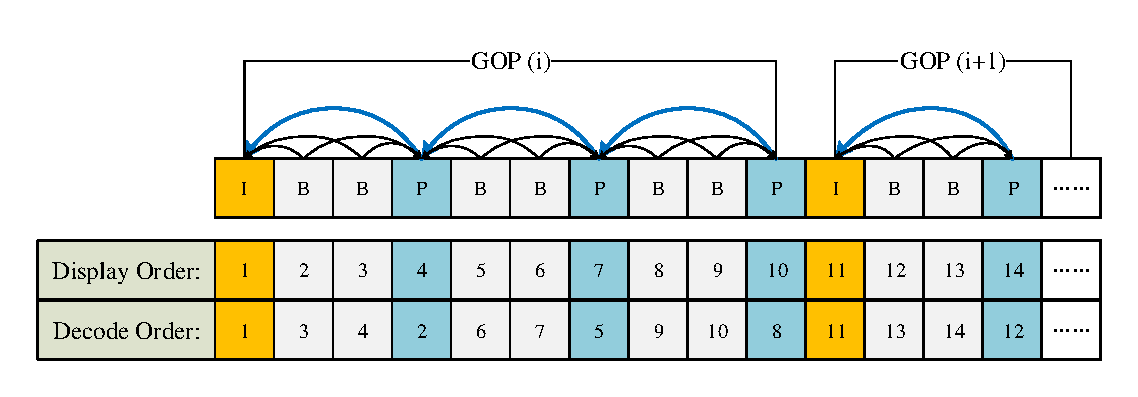
\includegraphics[width=0.48\textwidth]{photo/H264_IPB.pdf}
\caption{A sample of GOPs in H.264}
\label{H264-IPB}
\end{figure}

H.264 is one of the advanced algorithms for this type of work. This coding technique is widely used on platforms such as YouTube because it has higher compression ratio and lower complexity than its predecessor. For the HD video mentioned earlier, H.264 can reduce its size by about 10 times, only 443.27MB.

\subsection{Approximate Storage}
Approximate Storage is another way outside of traditional methods of trading off the limited resource budget with the costly reliability requirements, which recently receives more attentions since data centers are faced with storage pressure from the ever-increasing data.

It loosens the requirement of storage reliability by allowing some quality loss of specific data. Therefore, programmers can specify the importance of the data segments and assign them to different storage blocks. The critical data is still safe because they are stored and redundantly backed up by expensive and highly reliable storage devices. Meanwhile, non-critical data is exposed to error, thus increasing storage density and saving cost.

However, it is too naive to store data in approximate storage units indiscriminately. Related research [] shows that this can lead to unacceptable data pollution. To ensure data quality in this case, higher error correction costs are required resulting in an increase in overall storage costs.

In the storage of video data, as described in \ref{video storage}, the I frame is the key to decoding the entire GOP. An error in the I frame will cause a decoding error in the P frames and the B frames, and the data loss of the I frame will cause the entire GOP to be undecodable. In contrast, the error or loss of a P frame has less impact, while the B frame is most tolerant of errors because no other frame depends on it.

\subsection{Video Frame Recovery: Frame Interpolation}
In the circumstance of data loss, it's common to lose some frames and then the video is not complete. One easy way to solve this problem is to store consecutive frames in different disks, so the video is still good for displaying only with fewer frame rates. Another alternative is that we can actually recover the lost frames by applying the a technique named video frame interpolation.

Video frame interpolation is one of the basic video processing techniques, an attempt to synthetically produce one or more intermediate video frames from existing ones, the simple case being the interpolation of one frame given two consecutive video frames. This is a technique that can model natural motion within a video, and generate frames according to this modelling. Artificially increasing the frame-rate of videos enables the possibility of frame recovery. Optical flow is commonly addressed in the video frame interpolation problem. Optical flow is the pattern of apparent motion of objects, surfaces, and edges in a visual scene caused by the relative motion between an observer and a scene. Video frame interpolation algorithms typically estimate optical flow or its variations and use them to warp and blend original frames to produce interpolation results.

Recently, phase-based methods have shown promising results in applications such as motion and view extrapolation \cite{didyk2013joint}\cite{wadhwa2013phase}\cite{meyer2015phase}. These methods rely on the assumption that small motions can be encoded in the phase shift of an individual pixel¡¯s color. Meanwhile, deep learning approaches, and in particular Convolutional Neural Networks (CNNs), have set up new state-of-the-art results across many computer vision problems which also makes big improvements to frame interpolation. In neural networks, optical flow features are trained in a supervised setup mapping two frames to their ground truth optical flow field\cite{dosovitskiy2015flownet}\cite{ilg2017flownet}. Among them, a multi-scale network\cite{van2017frame} based on recent advances in spatial transformers and composite perceptual losses as well as a context-aware Synthesis approach\cite{niklaus2018context} have so far produced the best results in terms of PSNR and middlebury benchmark respectively.

All the frame interpolation method are based on that we have the input of full images of two consecutive frames (maybe one or two missing in the middle). However, in the popular coding format like H.264, only I frame have full image data of itself, and all the other image data is dependent on that in I frames. Without an I frame, the following ones that depend on it will go invalid and be impossible for recovery which means I frames require more storage overhead to ensure its integrity and reliability.

\subsection{Our Motivation}
Based on Table [], the existing erasure codes cannot meet the requirements of video applications in the cloud storage system due to the following reasons. First, existing erasure codes generally reach or exceed 3DFTS, and use more than 3 parity disks. However, the simultaneous damage of 3 disks is very rare, and the storage overhead paid for this is too large. Second, the existing erasure codes provide the same fault tolerance for all data without distinction, which results in the same reliability of important data that is sensitive to errors and data that is robust. To solve these two problems, we propose a new erasure code called approximation code. It provides different fault tolerance between important and non-critical data to reduce storage overhead and protect critical data better.

\section{Approximate Code}
In this section, we introduce the design of Approximate Codes and its properties through a simple example. In order to be general and easy to describe, we use fewer data blocks and more parity blocks (resulting in greater storage overhead). A more optimized parameter selection scheme for practical applications will be introduced in XXX.

\subsection{Design of Approximate Code}
In a system of $n$ disks, each disk can be divided into multiple sectors. We focus on the $r$ sectors of the same logical position of each device, and we treat these $r$ sectors as a chunk. The $r \times n$ sectors of $n$ chunks constitute a stripe, as shown in Figure \ref{TEST-chunk-sector} . We also use the term symbol in coding theory to refer to sectors. Since each strip is independent of the entire system, we only consider a single strip.

\begin{figure}[ht]
\centering
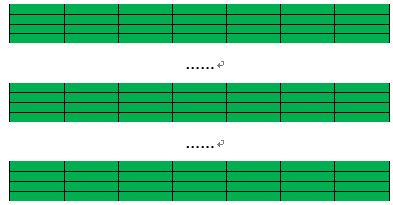
\includegraphics[width=0.4\textwidth]{photo/TEST-chunk-sector.JPG}
\caption{TEST--A sample of chunk and sector}
\label{TEST-chunk-sector}
\end{figure}

In the $n$ chunks of each stripe, $m$ ones are for coding and in the remaining $n-m$ chunks, we use $s \times t$ additional sectors for coding important data, where $s$ is the number of the columns and $t$ is the number of the rows.
Our design assumes that the parameters  $(n, m, s,t)$ are configurable parameters shus the constructor of the Approximate Code will be determined by these 4 parameters.
Although the choice of parameter $r$ is arbitrary, we recommend setting it to $r=s+h$.
The relevant instructions will be shown in \ref{Data Distribution}.
Meanwhile, we label $h=n-m-s$ as the number of columns of important data for convenience.
Figure \ref{apcode-7222-v4} shows an example of Approximate Codes with $n = 7$, $m = 2$, $s=2$ and $t = 2$, where we label the data disks with $d_{i,j}$, the important data parity sectors with $q_{i,j}$ and the normal parity sectors with $p_{i,j}$.

\begin{figure}[ht]
\centering
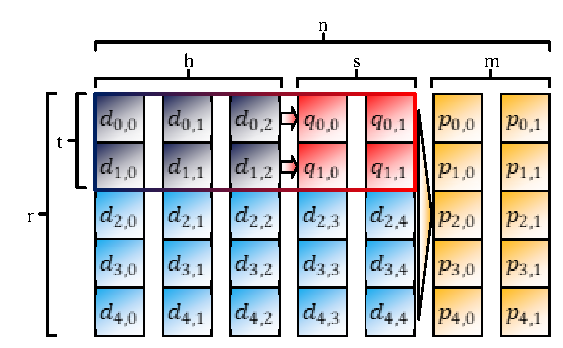
\includegraphics[width=0.4\textwidth]{photo/apcode-7222-v4.PDF}
\caption{A sample of Approximate Codes $(7,2,2,2)$ with 7 chunks where 2 of them are parity chunks (presented by orange) and 4 other sectors (presented by red) are designed for encoding important data. In this example, there are 6 sectors (presented by dark blue) for important data and 15 sectors (presented by light blue) for normal data.}
\label{apcode-7222-v4}
\end{figure}

A variety of erasure codes can be used for the encoding and decoding process of Approximate Codes. Here we only introduce our RS-based design as an example.
\hl{Approximate Codes based on other erasure code schemes include XOR-based codes or MSR codes will be introduced in Section }\ref{evaluation}.

\subsubsection{Encoding Process}
The encoding process can be divided into two phases: important coding phase and global coding phase.

In \emph{phase 1}, we use RS$(h+s,h)$ to encode $h$ groups of important data sectors and generate $s$ groups of parity sectors labeled with $q_{i,j}$. The calculation of $q_{i,j}$ are defined by equation \ref{q_ij}, where $\alpha_k$ is the coefficient in Galois Field (GF).
For example, $q_{1,1} = \alpha_0^2 d_{1,0} + \alpha_1^2 d_{1,1} + \alpha_2^2 d_{1,2}$.
As shown in the blod box in Figure \ref{apcode-7222-v2}, we use RS(5,3) in this phase.
\begin{equation}\label{q_ij}
    q_{i,j} = \sum_{k=0}^{h-1} \alpha_k^{j+1} d_{i,k}
\end{equation}

In \emph{phase 2}, we use RS$(n,n-m)$ to generate $m$ parity chunks labeled with $p_{i,j}$ from $n-m$ chunks consist of data sectors and important parity sectors. The calculation of $p_{i,j}$ are defined by equation \ref{p_ij_1} and \ref{p_ij_2}.
Despite the difference in expression, the encoding process for $p_{i,j(i<t)}$ and $p_{i,j(i \geqslant t)}$ are same on chunk level because we treat $q_{i,j}$ and $b_{i,j}$ as the same on chunk level.
For example, $p_{1,1} = \alpha_0^4 d_{1,0} + \alpha_1^4 d_{1,1} + \alpha_2^4 d_{1,2} + \alpha_3^4 q_{1,0} + \alpha_4^4 q_{1,1}$.
As shown in orange chunks in Figure \ref{apcode-7222-v2}, we use RS(7,5) in this phase.

\begin{equation}\label{p_ij_1}
    \mathop{p_{i,j}}\limits_{i<t} =
    \sum_{k=0}^{h-1} \alpha_k^{s+j+1} d_{i,k} +
    \sum_{l=0}^{s-1} \alpha_{l+h}^{s+j+1} q_{i,l}
\end{equation}
\begin{equation}\label{p_ij_2}
    \mathop{p_{i,j}}\limits_{i \geqslant t} =
    \sum_{k=0}^{n-m-1} \alpha_k^{s+j+1} d_{i,k}
\end{equation}



\subsection{Proof of Correctness}
\subsection{Data Distribution}\label{Data Distribution}
\subsection{Properties of Approximate Code}

\section{Evaluation}\label{evaluation}
\subsection{An Evaluation methodology}
\subsubsection{Erasure Codes in Our Comparisons}
\subsubsection{Platforms and Configurations}
\subsubsection{Metrics}
\subsubsection{Parameters and Assumption in Our Evaluation}


\subsection{Results}
\subsection{Analysis}
Illustrate why Approximate Code achieve high reliability with low cost
\section{Conclusion}
\section*{Acknowledgment}

\bibliographystyle{IEEEtrans}
\bibliography{paper}

\end{document}
